
  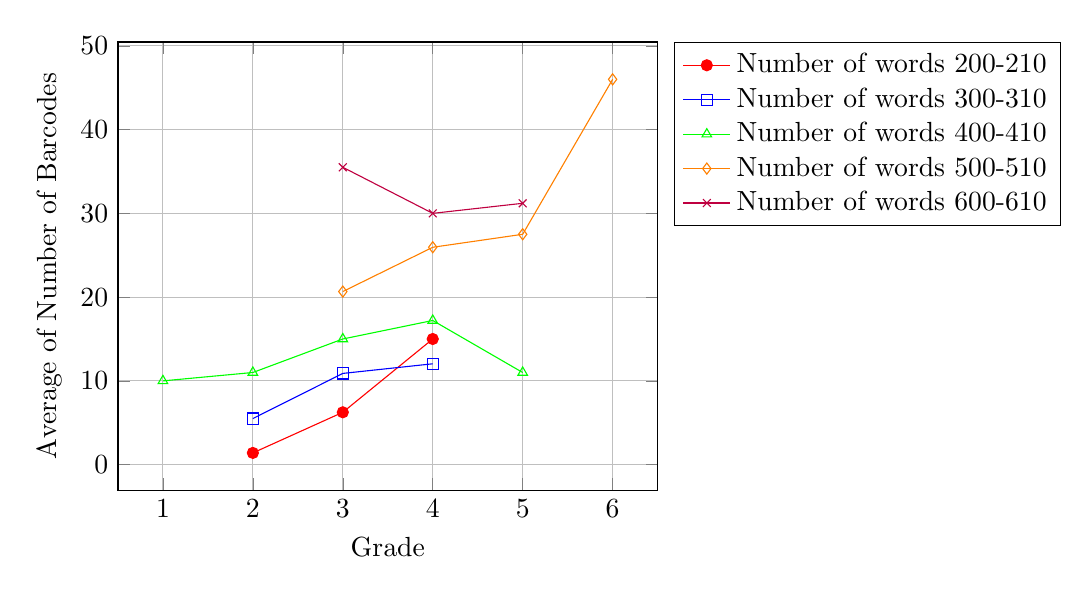
\begin{tikzpicture}
    \begin{axis}[
      xlabel={Grade},
      ylabel={Average of Number of Barcodes},
      legend pos=outer north east,
      grid=both,
    ]
    
    % Number of words 200-210
    \addplot[color=red,mark=*] coordinates {
      (2, 1.4)
      (3, 6.25)
      (4, 15.0)
    };
    
    % Number of words 300-310
    \addplot[color=blue,mark=square] coordinates {
      (2, 5.5)
      (3, 10.89)
      (4, 12.04)
    };
    
    % Number of words 400-410
    \addplot[color=green,mark=triangle] coordinates {
      (1, 10.0)
      (2, 11.0)
      (3, 15.0)
      (4, 17.21)
      (5, 11.0)
    };
    
    % Number of words 500-510
    \addplot[color=orange,mark=diamond] coordinates {
      (3, 20.66)
      (4, 25.95)
      (5, 27.5)
      (6, 46.0)
    };
    
    % Number of words 600-610
    \addplot[color=purple,mark=x] coordinates {
      (3, 35.5)
      (4, 30.0)
      (5, 31.2)
    };
    
    \legend{
      Number of words 200-210,
      Number of words 300-310,
      Number of words 400-410,
      Number of words 500-510,
      Number of words 600-610
    }
    
    \end{axis}
    \end{tikzpicture}
